%!TEX TS-program = xelatex
\documentclass[11pt]{article}

\usepackage[english]{babel}

\usepackage{amsmath,amssymb,amsfonts}
\usepackage[utf8]{inputenc}
\usepackage[T1]{fontenc}
\usepackage{stix2}
\usepackage[scaled]{helvet}
\usepackage[scaled]{inconsolata}

\usepackage{lastpage}

\usepackage{setspace}

\usepackage{ccicons}

\usepackage[hang,flushmargin]{footmisc}

\usepackage{geometry}

\setlength{\parindent}{0pt}
\setlength{\parskip}{6pt plus 2pt minus 1pt}

\usepackage{fancyhdr}
\renewcommand{\headrulewidth}{0pt}\providecommand{\tightlist}{%
  \setlength{\itemsep}{0pt}\setlength{\parskip}{0pt}}

\makeatletter
\newcounter{tableno}
\newenvironment{tablenos:no-prefix-table-caption}{
  \caption@ifcompatibility{}{
    \let\oldthetable\thetable
    \let\oldtheHtable\theHtable
    \renewcommand{\thetable}{tableno:\thetableno}
    \renewcommand{\theHtable}{tableno:\thetableno}
    \stepcounter{tableno}
    \captionsetup{labelformat=empty}
  }
}{
  \caption@ifcompatibility{}{
    \captionsetup{labelformat=default}
    \let\thetable\oldthetable
    \let\theHtable\oldtheHtable
    \addtocounter{table}{-1}
  }
}
\makeatother

\usepackage{array}
\newcommand{\PreserveBackslash}[1]{\let\temp=\\#1\let\\=\temp}
\let\PBS=\PreserveBackslash

\usepackage[breaklinks=true]{hyperref}
\hypersetup{colorlinks,%
citecolor=blue,%
filecolor=blue,%
linkcolor=blue,%
urlcolor=blue}
\usepackage{url}

\usepackage{caption}
\setcounter{secnumdepth}{0}
\usepackage{cleveref}

\usepackage{graphicx}
\makeatletter
\def\maxwidth{\ifdim\Gin@nat@width>\linewidth\linewidth
\else\Gin@nat@width\fi}
\makeatother
\let\Oldincludegraphics\includegraphics
\renewcommand{\includegraphics}[1]{\Oldincludegraphics[width=\maxwidth]{#1}}

\usepackage{longtable}
\usepackage{booktabs}

\usepackage{color}
\usepackage{fancyvrb}
\newcommand{\VerbBar}{|}
\newcommand{\VERB}{\Verb[commandchars=\\\{\}]}
\DefineVerbatimEnvironment{Highlighting}{Verbatim}{commandchars=\\\{\}}
% Add ',fontsize=\small' for more characters per line
\usepackage{framed}
\definecolor{shadecolor}{RGB}{248,248,248}
\newenvironment{Shaded}{\begin{snugshade}}{\end{snugshade}}
\newcommand{\KeywordTok}[1]{\textcolor[rgb]{0.13,0.29,0.53}{\textbf{#1}}}
\newcommand{\DataTypeTok}[1]{\textcolor[rgb]{0.13,0.29,0.53}{#1}}
\newcommand{\DecValTok}[1]{\textcolor[rgb]{0.00,0.00,0.81}{#1}}
\newcommand{\BaseNTok}[1]{\textcolor[rgb]{0.00,0.00,0.81}{#1}}
\newcommand{\FloatTok}[1]{\textcolor[rgb]{0.00,0.00,0.81}{#1}}
\newcommand{\ConstantTok}[1]{\textcolor[rgb]{0.00,0.00,0.00}{#1}}
\newcommand{\CharTok}[1]{\textcolor[rgb]{0.31,0.60,0.02}{#1}}
\newcommand{\SpecialCharTok}[1]{\textcolor[rgb]{0.00,0.00,0.00}{#1}}
\newcommand{\StringTok}[1]{\textcolor[rgb]{0.31,0.60,0.02}{#1}}
\newcommand{\VerbatimStringTok}[1]{\textcolor[rgb]{0.31,0.60,0.02}{#1}}
\newcommand{\SpecialStringTok}[1]{\textcolor[rgb]{0.31,0.60,0.02}{#1}}
\newcommand{\ImportTok}[1]{#1}
\newcommand{\CommentTok}[1]{\textcolor[rgb]{0.56,0.35,0.01}{\textit{#1}}}
\newcommand{\DocumentationTok}[1]{\textcolor[rgb]{0.56,0.35,0.01}{\textbf{\textit{#1}}}}
\newcommand{\AnnotationTok}[1]{\textcolor[rgb]{0.56,0.35,0.01}{\textbf{\textit{#1}}}}
\newcommand{\CommentVarTok}[1]{\textcolor[rgb]{0.56,0.35,0.01}{\textbf{\textit{#1}}}}
\newcommand{\OtherTok}[1]{\textcolor[rgb]{0.56,0.35,0.01}{#1}}
\newcommand{\FunctionTok}[1]{\textcolor[rgb]{0.00,0.00,0.00}{#1}}
\newcommand{\VariableTok}[1]{\textcolor[rgb]{0.00,0.00,0.00}{#1}}
\newcommand{\ControlFlowTok}[1]{\textcolor[rgb]{0.13,0.29,0.53}{\textbf{#1}}}
\newcommand{\OperatorTok}[1]{\textcolor[rgb]{0.81,0.36,0.00}{\textbf{#1}}}
\newcommand{\BuiltInTok}[1]{#1}
\newcommand{\ExtensionTok}[1]{#1}
\newcommand{\PreprocessorTok}[1]{\textcolor[rgb]{0.56,0.35,0.01}{\textit{#1}}}
\newcommand{\AttributeTok}[1]{\textcolor[rgb]{0.77,0.63,0.00}{#1}}
\newcommand{\RegionMarkerTok}[1]{#1}
\newcommand{\InformationTok}[1]{\textcolor[rgb]{0.56,0.35,0.01}{\textbf{\textit{#1}}}}
\newcommand{\WarningTok}[1]{\textcolor[rgb]{0.56,0.35,0.01}{\textbf{\textit{#1}}}}
\newcommand{\AlertTok}[1]{\textcolor[rgb]{0.94,0.16,0.16}{#1}}
\newcommand{\ErrorTok}[1]{\textcolor[rgb]{0.64,0.00,0.00}{\textbf{#1}}}
\newcommand{\NormalTok}[1]{#1}

\newlength{\cslhangindent}
\setlength{\cslhangindent}{1.5em}
\newlength{\csllabelwidth}
\setlength{\csllabelwidth}{3em}
\newenvironment{CSLReferences}[3] % #1 hanging-ident, #2 entry spacing
 {% don't indent paragraphs
  \setlength{\parindent}{0pt}
  % turn on hanging indent if param 1 is 1
  \ifodd #1 \everypar{\setlength{\hangindent}{\cslhangindent}}\ignorespaces\fi
  % set entry spacing
  \ifnum #2 > 0
  \setlength{\parskip}{#2\baselineskip}
  \fi
 }%
 {}
\usepackage{calc} % for \widthof, \maxof
\newcommand{\CSLBlock}[1]{#1\hfill\break}
\newcommand{\CSLLeftMargin}[1]{\parbox[t]{\maxof{\widthof{#1}}{\csllabelwidth}}{#1}}
\newcommand{\CSLRightInline}[1]{\parbox[t]{\linewidth}{#1}}
\newcommand{\CSLIndent}[1]{\hspace{\cslhangindent}#1}\geometry{verbose,letterpaper,tmargin=2.2cm,bmargin=2.2cm,lmargin=2.2cm,rmargin=2.2cm}

\usepackage{lineno}
\usepackage[nolists,noheads]{endfloat}

\pagestyle{plain}

\tolerance=1
\emergencystretch=\maxdimen
\hyphenpenalty=10000
\hbadness=10000

\doublespacing

\fancypagestyle{normal}
{
  \fancyhf{}
  \fancyfoot[R]{\footnotesize\sffamily\thepage\ of \pageref*{LastPage}}
}
\begin{document}
\raggedright
\thispagestyle{empty}
{\Large\bfseries\sffamily Forecasting the spatio-temporal uncoupling of
bumblebee-flower interaction networks}
\vskip 5em

%
\href{https://orcid.org/0000-0002-6506-6487}{Michael D.\,Catchen}%
%
\,\textsuperscript{1,2}\quad %
Paul\,CaraDonna%
%
\,\textsuperscript{3,4}\quad %
Jane E.\,Ogilvie%
%
\,\textsuperscript{3}\quad %
\href{https://orcid.org/0000-0001-9051-0597}{Francis\,Banville}%
%
\,\textsuperscript{5,6,2}\quad %
\href{https://orcid.org/0000-0002-2151-6693}{Dominique\,Caron}%
%
\,\textsuperscript{1,2}\quad %
\href{https://orcid.org/0000-0002-6248-3007}{Philippe\,Desjardins-Proulx}%
%
\,\textsuperscript{5,2}\quad %
\href{https://orcid.org/0000-0001-9019-0108}{Norma R.\,Forero-Muñoz}%
%
\,\textsuperscript{5,2}\quad %
\href{https://orcid.org/0000-0001-6075-8081}{Andrew\,Gonzalez}%
%
\,\textsuperscript{1,2}\quad %
\href{https://orcid.org/0000-0002-4498-7076}{Dominique\,Gravel}%
%
\,\textsuperscript{6,2}\quad %
\href{https://orcid.org/0000-0002-6004-4027}{Laura\,Pollock}%
%
\,\textsuperscript{1,2}\quad %
\href{https://orcid.org/0000-0002-0735-5184}{Timothée\,Poisot}%
%
\,\textsuperscript{5,2}\quad %
\href{https://orcid.org/0000-0001-6067-1349}{Tanya\,Strydom}%
%
\,\textsuperscript{5,2}\quad %
Julian\,Resasco%
%
\,\textsuperscript{7}

\textsuperscript{1}\,McGill University\quad \textsuperscript{2}\,Québec
Centre for Biodiversity Sciences\quad \textsuperscript{3}\,Rocky
Mountain Biological Laboratory\quad \textsuperscript{4}\,Chicago
Bontanic Garden\quad \textsuperscript{5}\,Université de
Montréal\quad \textsuperscript{6}\,Université de
Sherbrooke\quad \textsuperscript{7}\,University of Colorado Boulder


\textbf{Correspondance to:}\\
Michael D. Catchen --- \texttt{michael.catchen@mail.mcgill.ca}\\

\vfill
This work is released by its authors under a CC-BY 4.0 license\hfill\ccby\\
Last revision: \emph{\today}

\clearpage
\thispagestyle{empty}

\vfill


        {\bfseries Purpose:}\,This template provides a series of scripts
to render a markdown document into an interactive website and a series
of PDFs.\\%
        {\bfseries Motivation:}\,It makes collaborating on text with
GitHub easier, and means that we never need to think about the
output.\\%
        {\bfseries Internals:}\,GitHub actions and a series of python
scritpts. The markdown is handled with \texttt{pandoc}.\\%
    
\vfill

\clearpage
\linenumbers
\pagestyle{normal}

\hypertarget{abstract}{%
\subsection{Abstract}\label{abstract}}

Using a data set of {[}DESCRIBE EACH DATASET IN A NICE WAY{]}, we
predict a spatiotemporally explicit metaweb of interactions between
bumblebees (\emph{Bombus}) and wildflowers (within \emph{find clade}).
We integrate this data with crowdsourced occurrence data and climate
data to {[}best paint the picture of the Colorado bumblebee-plant
metaweb{]}. Using temporal climate data, we forecast how the
spatiotemporal overlap of interacting species will change under proposed
climate scenarios. We use this to estimate what interactions between
bees and plants need the most attention to prevent the spatiotemporal
decoupling of an interactions from threatening ecosystem functioning or
the persistence of a species.

\hypertarget{introduction}{%
\section{Introduction}\label{introduction}}

\begin{itemize}
\tightlist
\item
  We estimate the Colorado bumblebee/wild-flower pollination metaweb
  using network embedding.
\item
  Then decompose into spatial and temporally explicit network
  predictions
\item
  Finally suggest a priority of sampling to improve our understanding of
  this system.
\end{itemize}

\hypertarget{data}{%
\section{Data}\label{data}}

\hypertarget{methods}{%
\section{Methods}\label{methods}}

\textbf{\emph{Concept Fig}}

\hypertarget{metaweb-model}{%
\section{Metaweb Model}\label{metaweb-model}}

\hypertarget{phylogeny-construction}{%
\subsection{Phylogeny Construction}\label{phylogeny-construction}}

\hypertarget{feature-embedding}{%
\subsection{Feature Embedding}\label{feature-embedding}}

\hypertarget{relative-abundance}{%
\subsubsection{Relative Abundance}\label{relative-abundance}}

\hypertarget{phylogenetic-features}{%
\subsubsection{Phylogenetic features}\label{phylogenetic-features}}

\hypertarget{environmental-niche-features}{%
\subsubsection{Environmental niche
features}\label{environmental-niche-features}}

\hypertarget{temporal-niche-features}{%
\subsubsection{Temporal niche features}\label{temporal-niche-features}}

\hypertarget{metaweb-model-fitting-and-validation}{%
\subsection{Metaweb Model Fitting and
Validation}\label{metaweb-model-fitting-and-validation}}

\textbf{\emph{Figure 2: Model Fit Figure}}
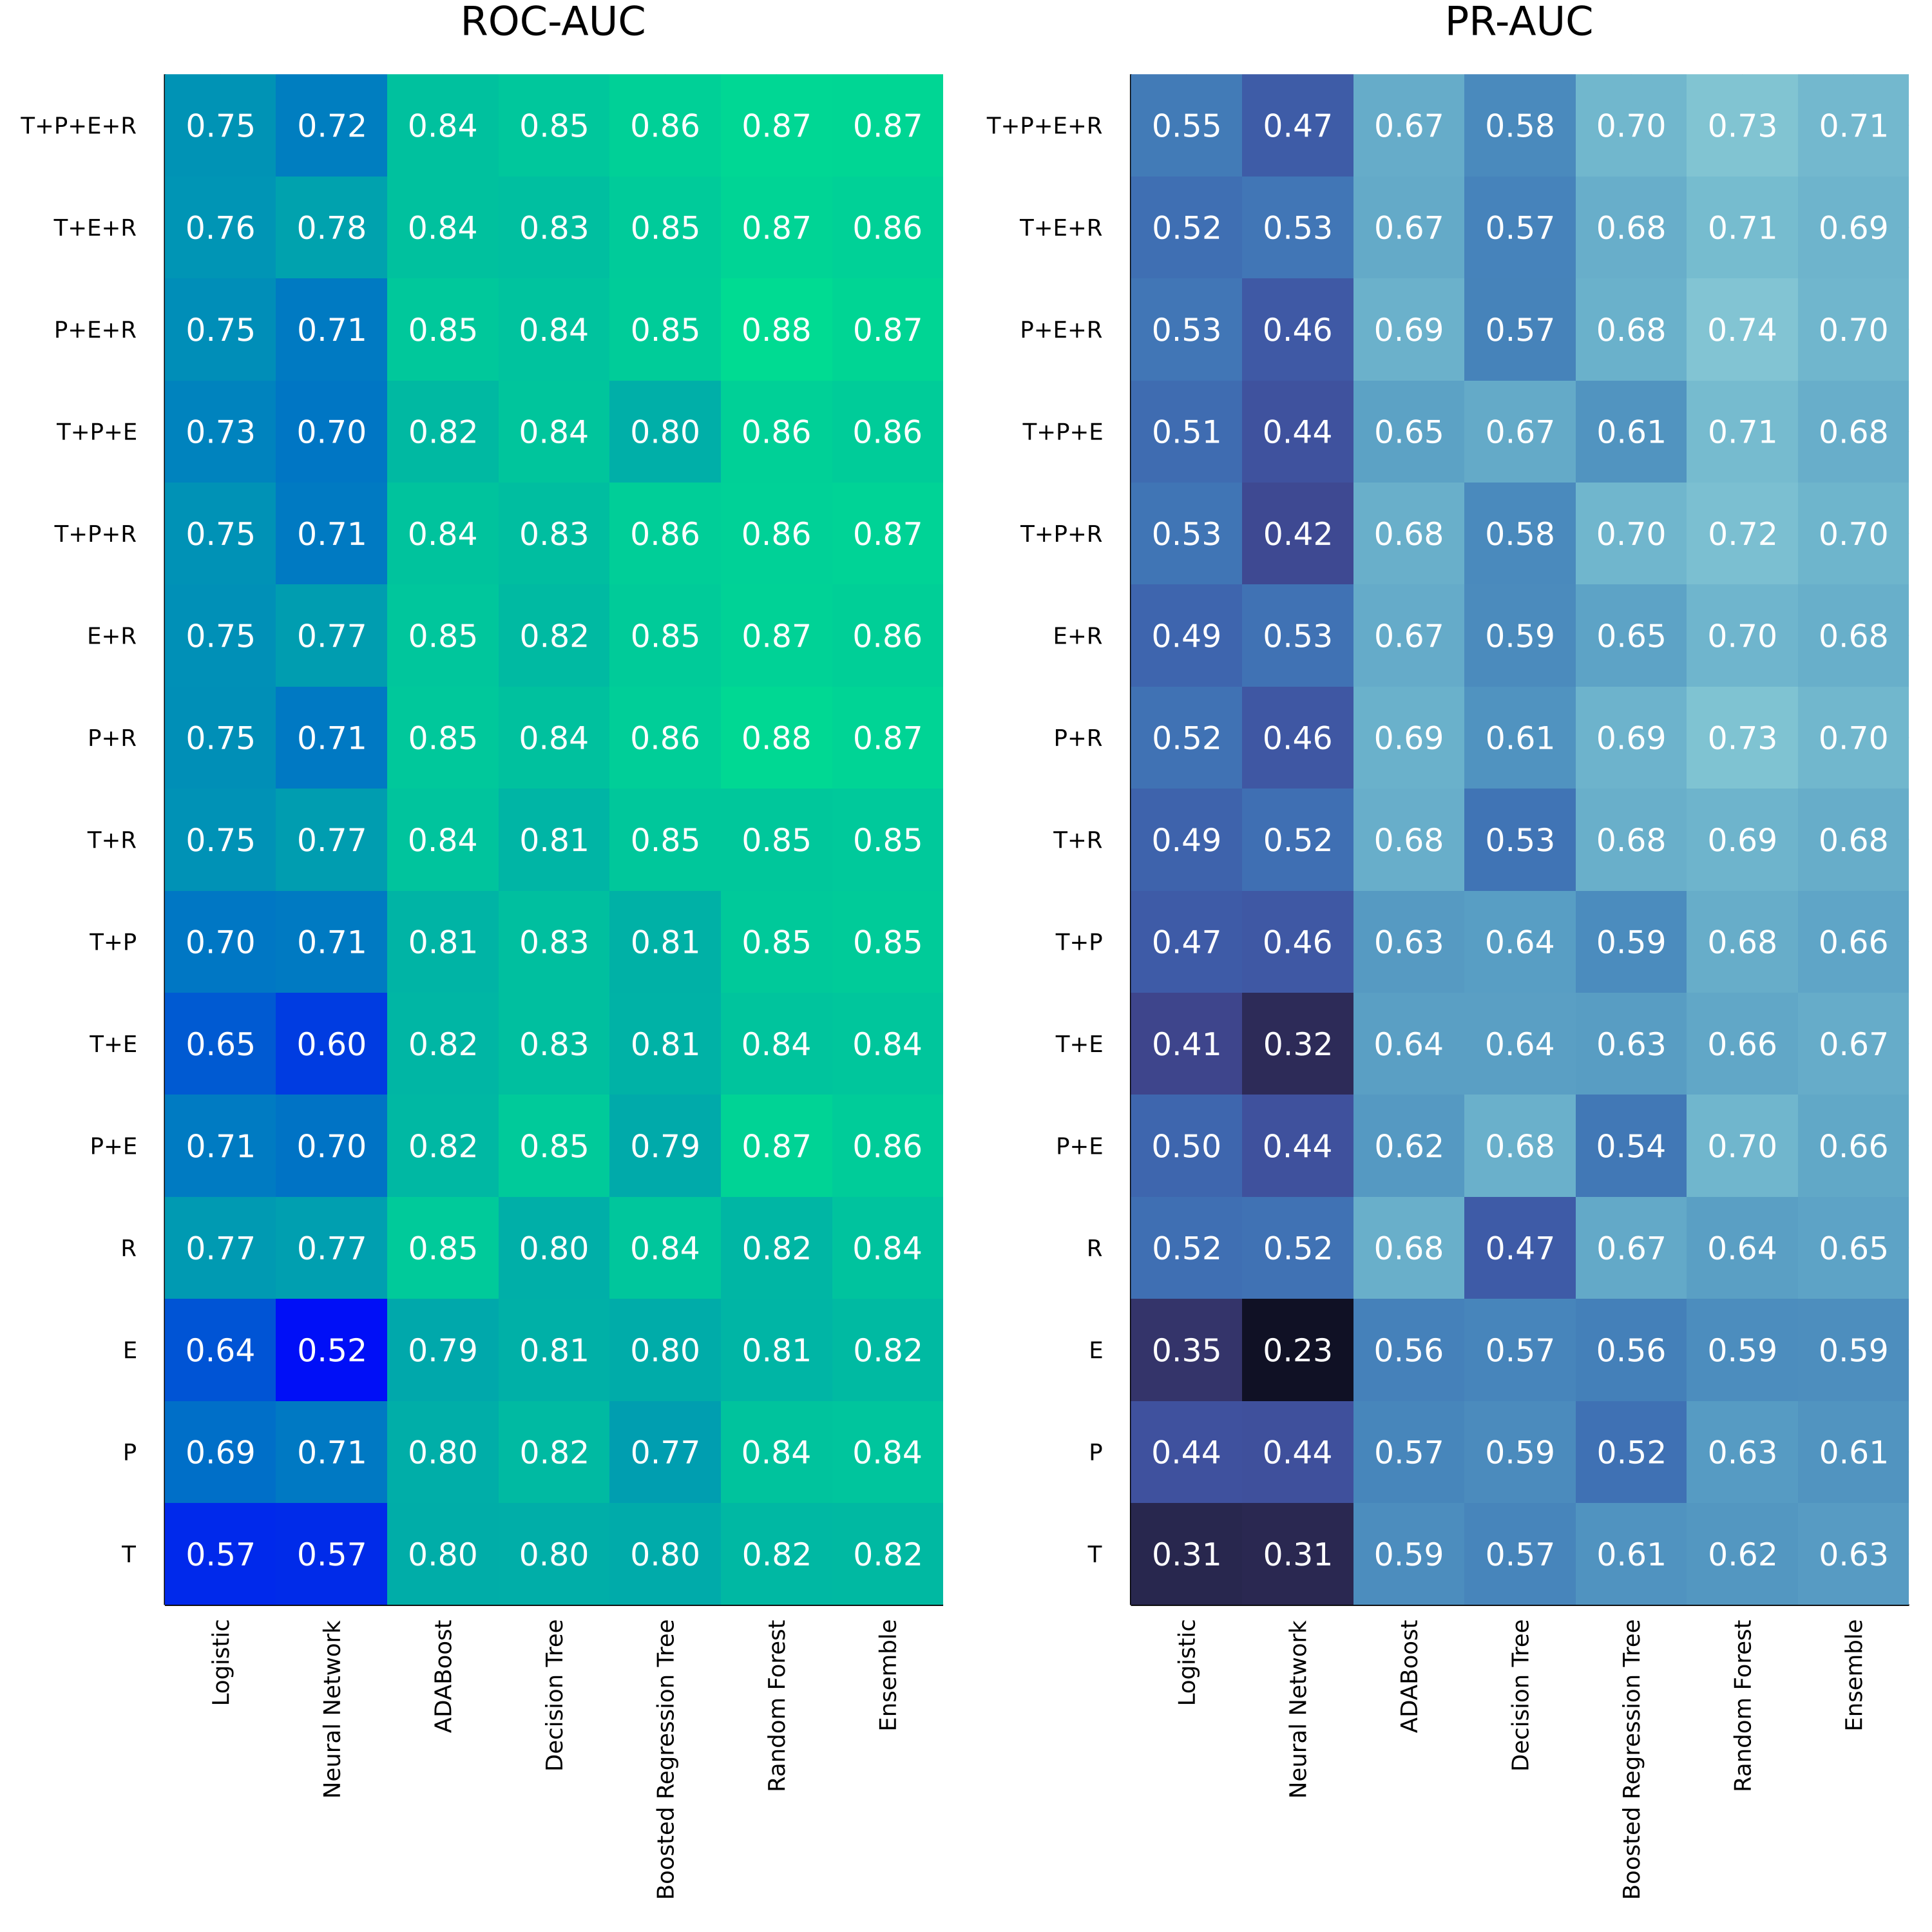
\includegraphics{./figures/PR_ROC.png} \# Spatiotemporally Explicit
Networks

Now that we have a metaweb\ldots..

\textbf{\emph{Figure 3: Maps over time figure and Prob(Connectance)
vs.~Month figure }}

\hypertarget{sampling-prioiritization}{%
\section{Sampling Prioiritization}\label{sampling-prioiritization}}

\textbf{\emph{Figure 4: Uncertainty and sampling priority map}}

\hypertarget{discussion}{%
\section{Discussion}\label{discussion}}

\end{document}
